\subsubsection{Turbine à vapeur}
\label{exo_turbine_vapeur}

	\begin{figure}
		\begin{center}
			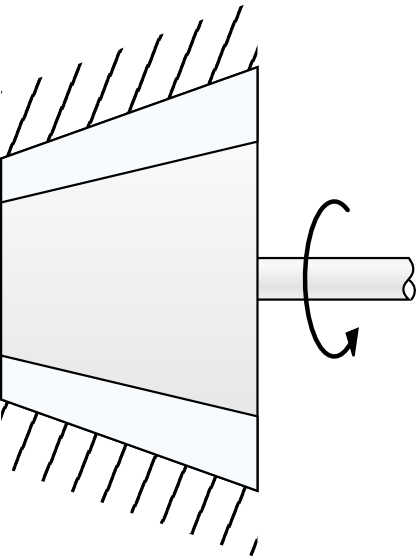
\includegraphics[height=0.45\textwidth, max height=0.5\columnwidth]{images/symbole_turbine.png}
			\hspace{0.5cm}
			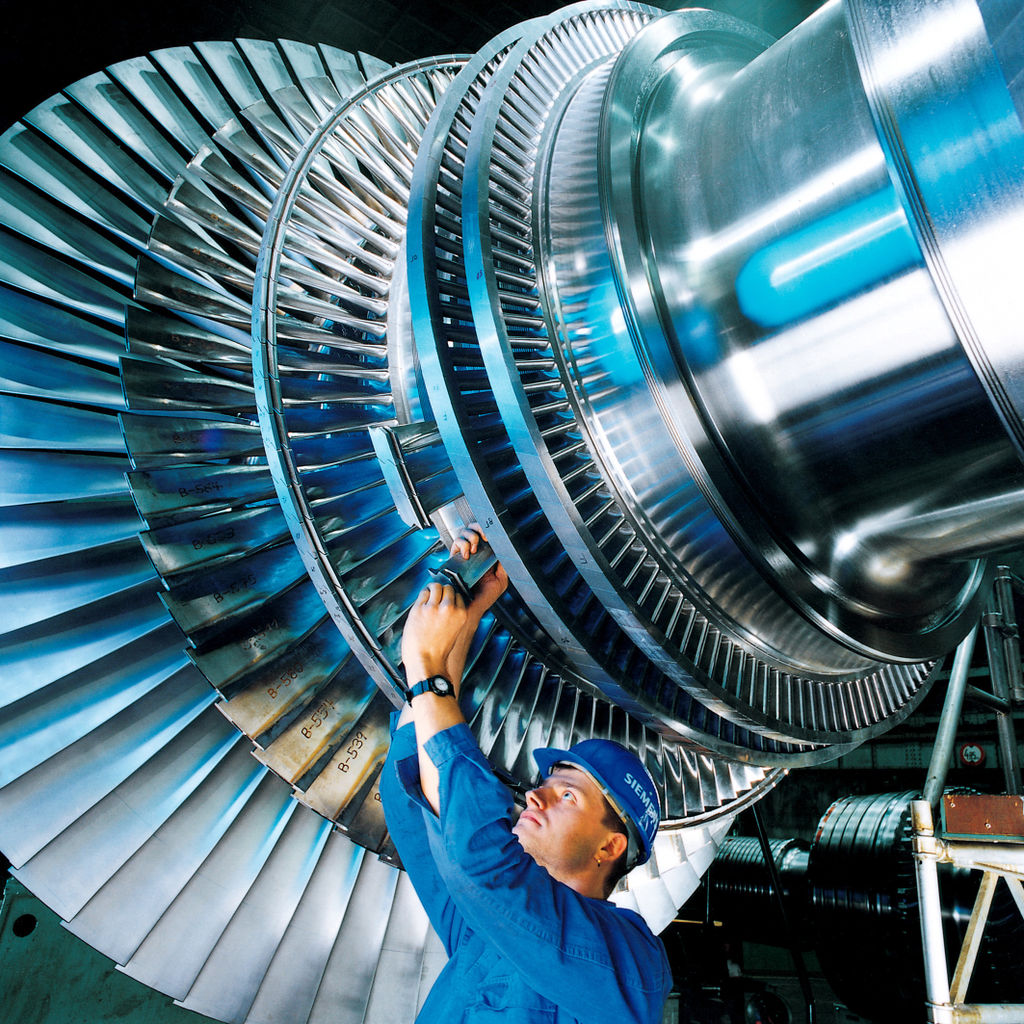
\includegraphics[height=0.45\textwidth, max height=0.5\columnwidth]{images/steam_turbine_siemens.jpg}
		\end{center}
		\supercaption{Schéma de principe et photo d’une turbine à vapeur.}{schéma \cczero \oc ; \wcfile{Dampfturbine Laeufer01.jpg}{photo} \ccbysa Siemens Pressebild}
		\label{fig_turbine_vapeur}
	\end{figure}
	
	Une turbine à vapeur (\cref{fig_turbine_vapeur}) équipe une petite centrale électrique alimentée par la combustion de matières organiques végétales.
	
	À l’entrée de la turbine, la vapeur a les propriétés suivantes :
		
	\begin{itemize}
		\item Pression : 		\tab \SI{45}{\bar}
		\item Température : 	\tab \SI{400}{\degreeCelsius}
		\item Volume spécifique : 	\tab \SI{0,06477}{\metre\cubed\per\kilogram}
		\item Énergie interne : 	\tab \SI{2914,2}{\kilo\joule\per\kilogram}
	\end{itemize}
	
	À la sortie de la turbine, on mesure les propriétés suivantes :
		
	\begin{itemize}
		\item Pression : 			\tab \SI{0,75}{\bar}
		\item Température : 		\tab \SI{91,61}{\degreeCelsius}
		\item Volume spécifique : 	\tab \SI{2,122}{\metre\cubed\per\kilogram}
		\item Énergie interne : 	\tab \SI{2316,3}{\kilo\joule\per\kilogram}
	\end{itemize}
	
	Les pertes sous forme de chaleur sont négligeables.
	
	\begin{enumerate}
		\item Quelle est la puissance spécifique sous forme de travail qui est dégagée par la turbine ?
		\item Quel débit de vapeur faut-il admettre pour générer une puissance de~\SI{4}{\mega\watt} ?
	\end{enumerate}



\subsubsection{Génératrice de courant électrique}
\label{exo_generatrice_electrique}

	Dans une installation portative génératrice d’électricité, le générateur électrique est entraîné par un axe mécanique. Le long de cet axe, on trouve un compresseur à air et une turbine (\cref{fig_elgen}).
	\begin{figure}
		\begin{center}
			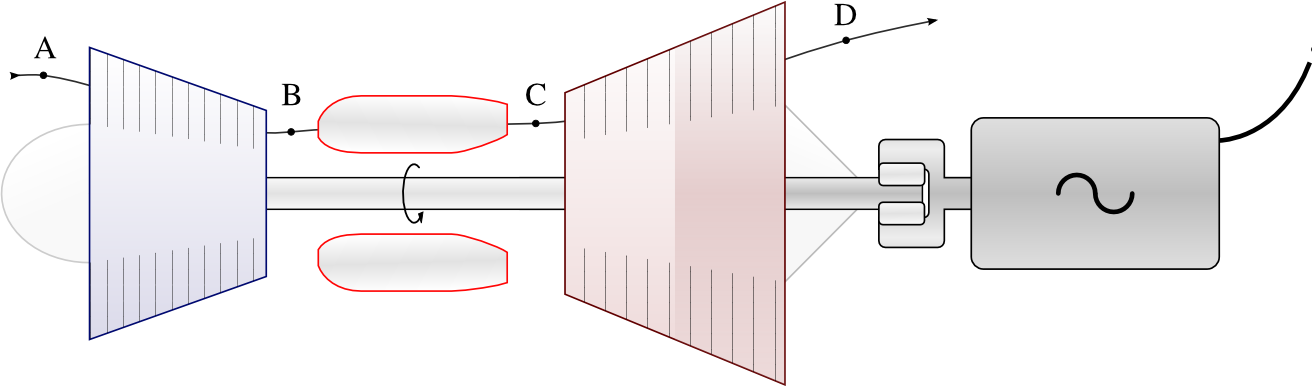
\includegraphics[width=\textwidth]{images/circuit_generateur.png}
		\end{center}
		\supercaption{Schéma de principe d’une turbomachine génératrice d’électricité.}{\ccbysa \olivier}
		\label{fig_elgen}
	\end{figure}	
	Ce type d’installation, parfois simplement nommé «~turbine à gaz~», est particulièrement compact et efficace ; il nécessite par contre l’emploi de carburants raffinés.

	Le compresseur porte l’air depuis les conditions atmosphériques jusqu’à une forte pression et une haute température.
	
	Entrée du compresseur :		
	\begin{itemize}
		\item Pression : 				\tab \SI{1}{\bar}
		\item Volume spécifique : 	\tab \SI{0,751}{\metre\cubed\per\kilogram}
		\item Énergie interne : 	\tab \SI{206,78}{\kilo\joule\per\kilogram}
	\end{itemize}

	Sortie du compresseur :		
	\begin{itemize}
		\item Pression : 				\tab \SI{35}{\bar}
		\item Volume spécifique : 	\tab \SI{6,602e-2}{\metre\cubed\per\kilogram}
		\item Énergie interne : 	\tab \SI{578,13}{\kilo\joule\per\kilogram}
	\end{itemize}

	Entre le compresseur et la turbine, la chambre de combustion porte les gaz à très haute température. La combustion se fait à pression constante ; elle porte les gaz à un volume spécifique de~\SI{0,1168}{\metre\cubed\per\kilogram} et à une énergie interne de~\SI{1028,8}{\kilo\joule\per\kilogram}.
	
	À la sortie de la turbine, les gaz sont prêts à être refroidis dans un circuit d’échappement catalytique destiné, entre autres, à réduire les émissions de bruit.
	
	Sortie de la turbine :		
	\begin{itemize}
		\item Pression : 				\tab \SI{1,2}{\bar}
		\item Volume spécifique : 	\tab \SI{1,526}{\metre\cubed\per\kilogram}
		\item Énergie interne : 	\tab \SI{460,88}{\kilo\joule\per\kilogram}
	\end{itemize}

	Le débit d’air admis dans la machine est de~\SI{8}{\kilogram\per\second} ; les variations de son énergie mécanique sont quasi nulles.\\
	Les déperditions de chaleur par les parois de la machine sont négligeables. Les pertes mécaniques sont de l’ordre de~\SI{2}{\percent} de la puissance transmise au générateur. Le générateur électrique lui-même a une efficacité de~\SI{85}{\percent}.

	\begin{enumerate}
		\item Quelle puissance est perdue ou gagnée par l’air dans le compresseur ?
		\item Quelle puissance est perdue ou gagnée par l’air dans la turbine ?
		\item Quelle est la puissance électrique générée par l’installation ?
		\item Représentez l’évolution suivie par l’air lorqu’il traverse le moteur sur un diagramme pression-volume, de façon qualitative (c’est-à-dire sans représenter les valeurs numériques).
		\item Quelle est la puissance perdue sous forme de chaleur avec les gaz d’échappement ?\\
				\small{\relax[indice : c’est la chaleur que les gaz devraient perdre pour retrouver leur état à l’entrée du compresseur]}
	\end{enumerate}


\subsubsection{Chaudière à vapeur}
\label{exo_chaudiere_vapeur}

	Une centrale fournit de l’électricité ainsi que de la chaleur industrielle et domestique à partir de la combustion de déchets ménagers (installation dite \textit{de cogénération}). Elle est équipée d’un circuit d’eau qui reçoit une partie de la chaleur dégagée par la combustion, à pression constante, dans une chaudière.
	
	L’eau pénètre dans la chaudière (\cref{fig_boiler}) à l’état liquide, pressurisée à~\SI{70,5}{\bar}. Son énergie interne est alors de~\SI{1160,2}{\kilo\joule\per\kilogram}. On souhaite alimenter la turbine avec \SI{317}{\tonne\per\hour} de vapeur à enthalpie de~\SI{3595,9}{\kilo\joule\per\kilogram}.

	\begin{figure}
		\begin{center}
			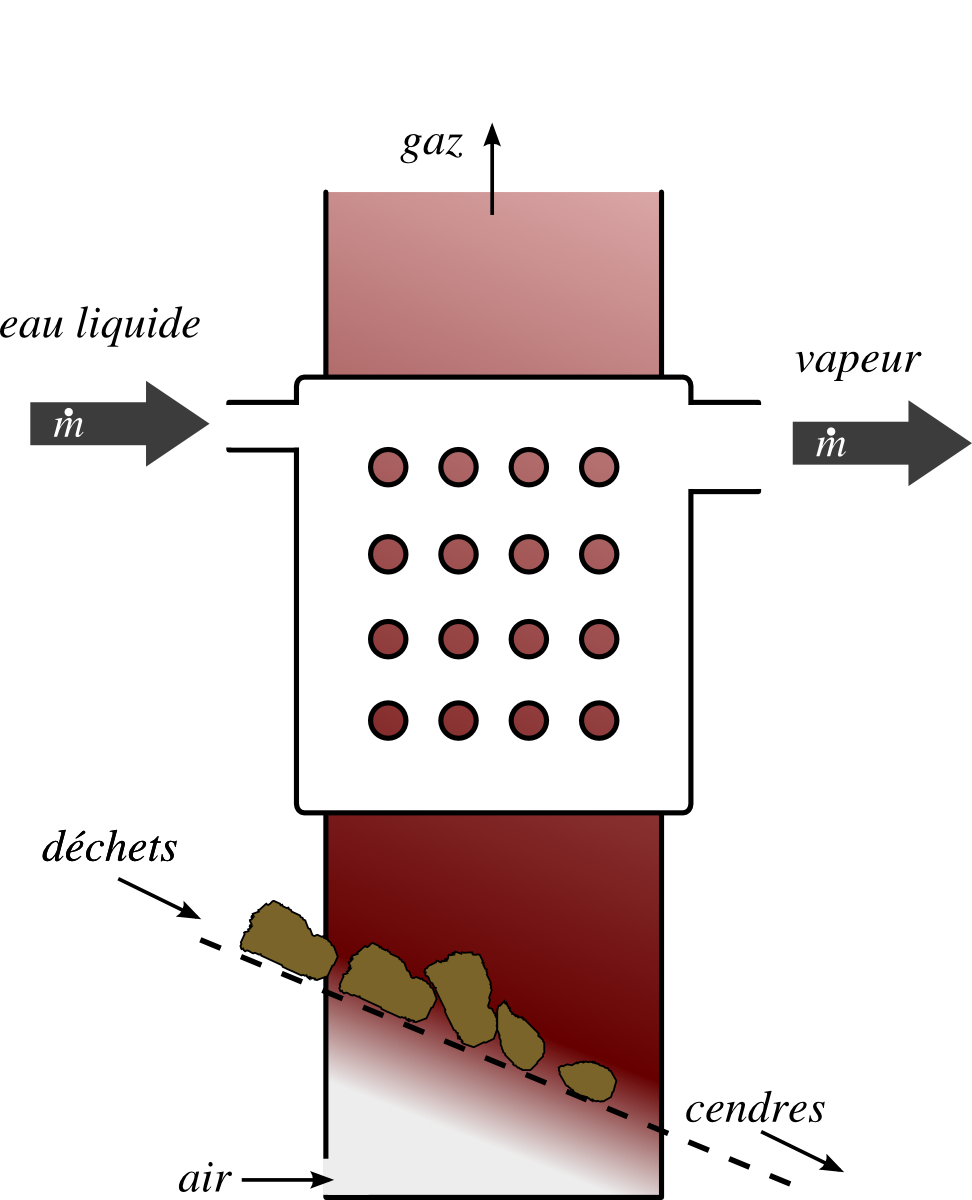
\includegraphics[height=10cm, max width=0.9\columnwidth]{images/boiler.png}
		\end{center}
		\supercaption{Schéma de principe d’une chaudière fonctionnant à partir de la combustion de déchets.}{schéma \cczero \oc}
		\label{fig_boiler}
	\end{figure}
	
	La combustion des déchets ménagers génère entre \num{9} et~\SI{11}{\mega\joule\per\kilogram} de chaleur ; l’efficacité de la chaudière est de~\SI{76}{\percent}.
	
	Quel est le débit minimum de déchets que la centrale doit recevoir pour assurer la production de vapeur ?
	

\subsubsection{Tuyère de turboréacteur}
\label{exo_tuyere_turboreacteur}

	Dans la tuyère d’un petit turboréacteur, la pression de l’air chute tandis que sa vitesse augmente. La tuyère (\cref{fig_nozzle}) est un élément sans aucune pièce mobile : aucun transfert de travail n’y est effectué. Les pertes en chaleur y sont négligeables et le débit d’air est de~\SI{26}{\kilogram\per\second}.

	\begin{figure}
		\begin{center}
			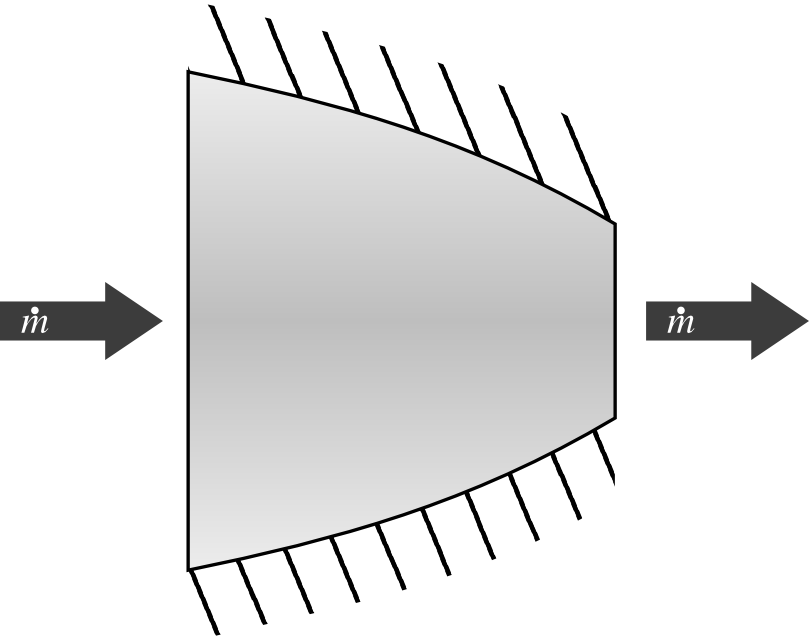
\includegraphics[height=0.35\textwidth, max height=0.5\columnwidth]{images/symbole_tuyere.png}
			\hspace{0.3cm}
			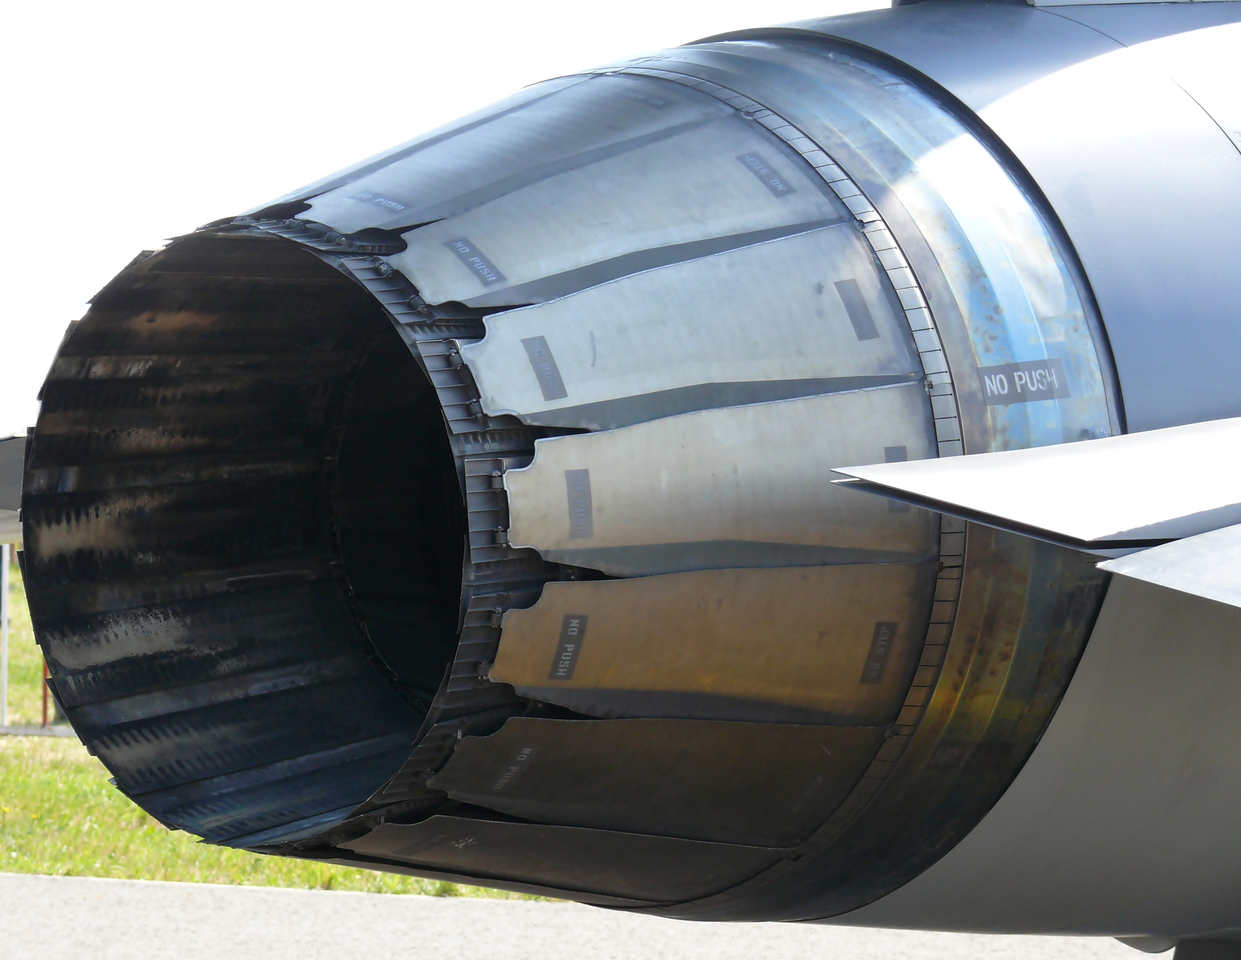
\includegraphics[height=0.35\textwidth, max height=0.5\columnwidth]{images/nozzle_f100.jpg}
		\end{center}
		\supercaption{Schéma de principe d’une tuyère et installation (avec géométrie variable) sur le moteur \textit{Pratt \& Whitney} F100 d’un Lockheed Martin F-16.}{schéma \cczero \oc ; \wcfile{F-16 Exhaust.JPG}{Photo} : \ccbysa Ad Meskens}
		\label{fig_nozzle}
	\end{figure}

	
	À l’entrée, on mesure les caractéristiques suivantes :
		
	\begin{itemize}
		\item enthalpie spécifique 		\tab \SI{1092}{\kilo\joule\per\kilogram}
		\item vitesse 							\tab \SI{10}{\metre\per\second}
		\item température 					\tab \SI{950}{\kelvin}
		\item volume spécifique 			\tab \SI{1,36}{\metre\cubed\per\kilogram}
		\item pression 						\tab \SI{2,28}{\bar}
		\item énergie interne 				\tab \SI{781,85}{\kilo\joule\per\kilogram}
	\end{itemize}

	À la sortie, l’air est redescendu à pression atmosphérique (\SI{1}{\bar}). On prédit\footnote{Il faut attendre le \coursquatre pour que nous puissions effectuer ces «~prédictions~».} que les caractéristiques de l’air atteindront :
		
	\begin{itemize}
		\item température  				\tab \SI{780,2}{\kelvin}
		\item volume spécifique  		\tab \SI{2,55}{\metre\cubed\per\kilogram}
		\item énergie interne  			\tab \SI{642,1}{\kilo\joule\per\kilogram}
	\end{itemize}


	\begin{enumerate}
		\item À quelle vitesse les gaz sont-ils éjectés ?
		\item Quels sont les débits volumiques d’air à l’entrée et à la sortie de la tuyère ?
	\end{enumerate}
	

\subsubsection{Turbine à eau}
\label{exo_turbine_eau}

	Un/e ingénieur/e travaille sur un projet de petite installation hydroélectrique. L’objectif est d’exploiter la circulation d’un cours d’eau (\SI{12}{\metre\cubed\per\second}) avec une turbine reliée à un générateur électrique (\cref{fig_water_turbine_1}).
	
	\begin{figure}
		\begin{center}
			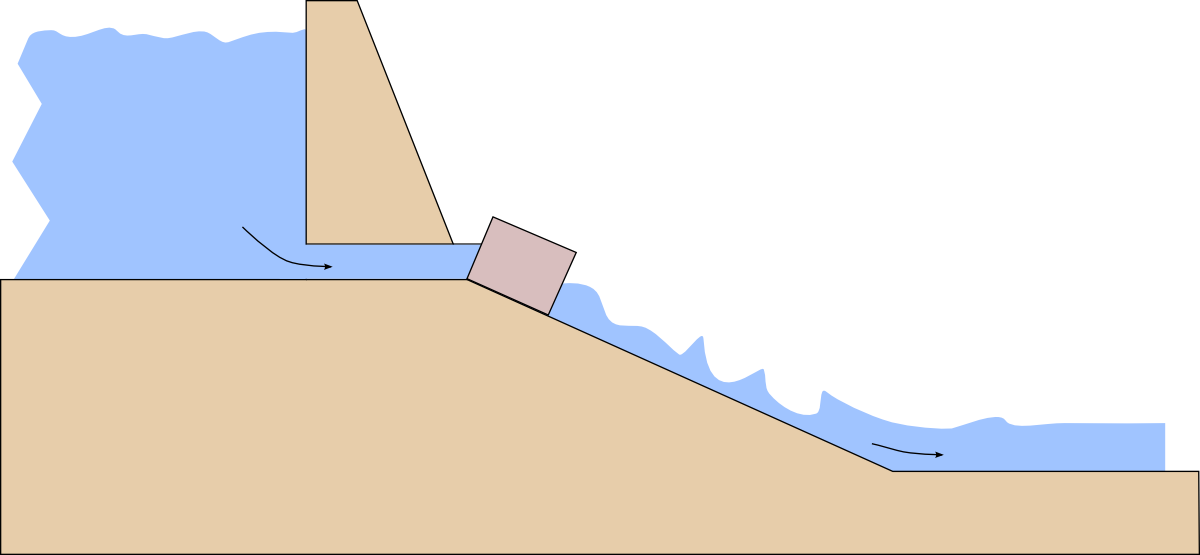
\includegraphics[width=10cm]{images/water_turbine_1.png}
		\end{center}
		\supercaption{Schéma de principe d’une installation génératrice hydraulique.}{schéma \cczero \oc}
		\label{fig_water_turbine_1}
	\end{figure}
	
	À l’état liquide, l’eau est essentiellement incompressible (c’est-à-dire que sa masse volumique ne varie pas lorsque sa pression change). Son énergie interne varie également de façon négligeable pendant les compressions et détentes adiabatiques.
	
	L’ingénieur/e pense tout d’abord positionner la turbine au pied d’une retenue d’eau, où la pression est de~\SI{4}{\bar} et la vitesse quasi-nulle. Le dénivelé parcouru par l’eau à travers la turbine est de~\SI{2}{\metre} et sa vitesse d’éjection est de~\SI{4}{\metre\per\second}, à pression atmosphérique (\SI{1}{\bar}).
	
	\begin{enumerate}
		\item Quelle puissance la turbine pourrait-elle transmettre à la génératrice ?
	\end{enumerate}

	L’ingénieur/e étudie ensuite une configuration différente (\cref{fig_water_turbine_2}). La turbine garderait les mêmes caractéristiques, mais serait positionnée plus en aval de la retenue d’eau (décalage de~\SI{25}{\metre} horizontalement et autant verticalement).
	
	\begin{figure}
		\begin{center}
			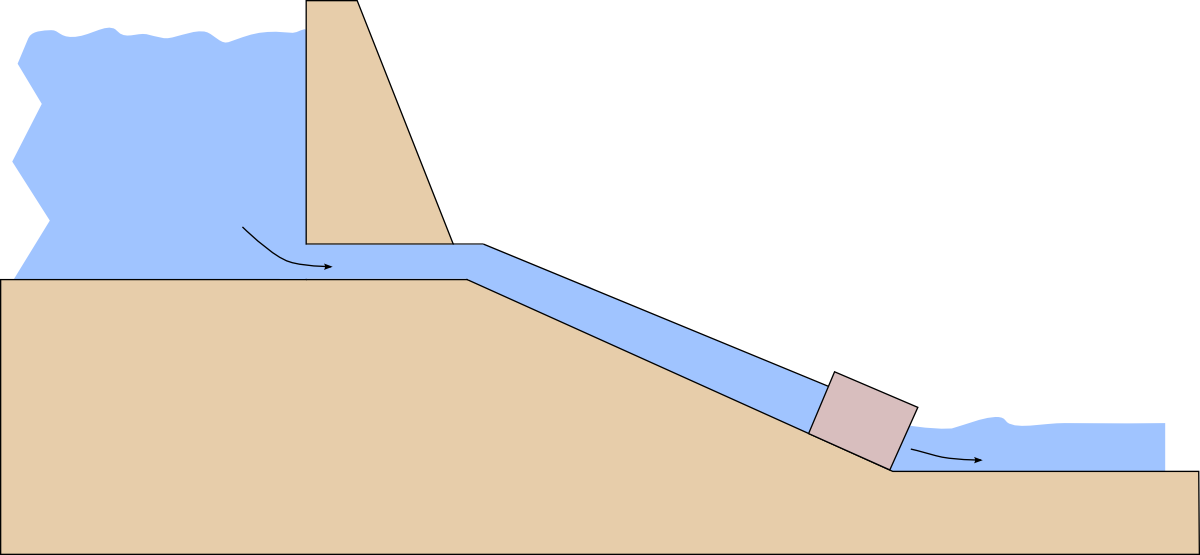
\includegraphics[width=10cm]{images/water_turbine_2.png}
		\end{center}
		\supercaption{Schéma de principe de l’installation modifiée. Une conduite rigide amène l’eau jusqu’à la turbine placée plus en contrebas.}{schéma \cczero \oc}
		\label{fig_water_turbine_2}
	\end{figure}

	\begin{enumerate}
		\shift{1}
		\item Quelle serait alors la puissance transmise ?
	\end{enumerate}


\subsubsection{Système de post-combustion}
\label{exo_postcombustion}

	Pour augmenter la poussée qu’elle génère, on modifie la tuyère de l’exercice~\ref{exo_tuyere_turboreacteur} pour y ajouter un appareillage de réchauffe (la réchauffe est souvent appelée \vocab{postcombustion}, cf. \S\ref{ch_postcombustion} p.\pageref{ch_postcombustion}). Il s’agit d’un ensemble de brûleurs qui permettent une seconde combustion de carburant dans le moteur, juste avant que l’air n’entame sa détente dans la tuyère (\cref{fig_afterburner}). Après la seconde combustion, l’air effectue sa détente et son accélération jusqu’à la pression atmosphérique.

	\begin{figure}
		\begin{center}
			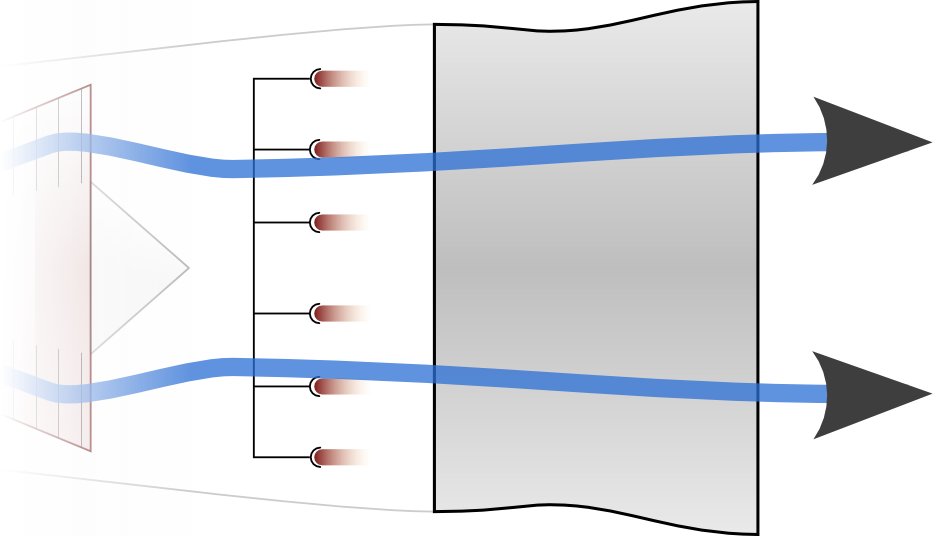
\includegraphics[width=9cm, max width=0.8\columnwidth]{images/postcombustion.png}
		\end{center}
		\supercaption{Schéma de principe d’un système de postcombustion. Son fonctionnement est étudié en \S\ref{ch_postcombustion} p.\pageref{ch_postcombustion}}{\ccbysa \olivier}
		\label{fig_afterburner}
	\end{figure}

	À l’entrée, les conditions sont identiques à celles indiquées dans l’exercice~\ref{exo_tuyere_turboreacteur}.
	
	La puissance spécifique apportée sous forme de chaleur par les brûleurs atteint \SI{1322,5}{\kilo\joule\per\kilogram}. Le carburant brûlé a une capacité calorifique massique de~\SI{30}{\mega\joule\per\kilogram}. La combustion se fait à pression constante et elle n’augmente pas l’énergie cinétique du gaz.
	
	Lorsque l’air termine son accélération, on peut prédire son énergie interne à~\SI{1412,8}{\kilo\joule\per\kilogram} et son volume spécifique à~\SI{5,61}{\metre\cubed\per\kilogram}.
	
	\begin{enumerate}
		\item Quelle est l’augmentation de la vitesse d’éjection (et ainsi de la poussée) générée par la postcombustion ?
		\item Quel débit de carburant doit-on injecter dans les brûleurs, en~\si[per-mode=symbol]{\kilogram\per\hour} ?
		\item Quel est le débit volumique d’air après son accélération finale ?
		\item Quelle est l’efficacité de la postcombustion, c’est à dire le rapport entre l’augmentation de l’énergie cinétique des gaz et l’augmentation de la puissance à apporter sous forme de chaleur ?
	\end{enumerate}

	
\subsubsection{Turbine à vapeur}
\label{exo_turbine_vapeur_2}

	Une turbine à vapeur de petite taille dégage \SI{500}{\kilo\watt} de puissance, avec un débit massique de~\SI{1,35}{\kilogram\per\second}.
	
	La vitesse moyenne de la vapeur est de~\SI{60}{\metre\per\second} à l’entrée, \SI{360}{\metre\per\second} à la sortie ; elle gagne \SI{3}{\metre} d’altitude au cours du parcours. La perte de chaleur représente \SI{3}{\kilo\watt}.
	
	
	\begin{enumerate}
		\item Quelles sont les variations d’énergie cinétique, d’énergie potentielle et d’enthalpie de la vapeur, lorsqu’elle traverse la turbine ?
		\item Puisque la perte de chaleur est de~\SI{3}{\kilo\watt}, pourquoi ne pas isoler thermiquement la turbine pour pouvoir récupérer cette puissance sous forme de travail ?
	\end{enumerate}
	

	
\subsubsection{Turbines théorique et réelle}
\label{exo_detente_turbine_turbomoteur}

	Dans la turbine libre du turbomoteur d’un hélicoptère, l’air est détendu pour extraire du travail transmis aux deux rotors. Les caractéristiques sont les suivantes :
	
	\begin{itemize}
		\item Débit de masse : 		\tab \SI{2}{\kilogram\per\second}
		\item Pertes sous forme de chaleur : négligeables
		\item Entrée :  				\tab \SI{4}{\bar} et~\SI{0,41}{\metre\cubed\per\kilogram}
		\item Pression de sortie : \tab \SI{1,1}{\bar}
	\end{itemize}
	
	Dans le cas le plus favorable, la détente se ferait de façon réversible et l’air suivrait une relation de type $p v^{\num{1,4}} = k$ (où $k$ est une constante).
	
	\begin{enumerate}
		\item Quelles conditions devraient être respectées pour que la détente soit réversible ?
		\item Quelle serait la puissance fournie par la turbine dans ce cas ?
	\end{enumerate}
	
	En pratique, il est constaté que la puissance fournie par la turbine est de~\SI{20}{\percent} inférieure à la valeur calculée plus haut. Un/e ingénieur/e installe des sondes à l’entrée et à la sortie de la turbine et constate que la pression y atteint pourtant bien les valeurs prévues en théorie. Il/elle mesure également le transfert de chaleur de l’air vers la turbine et confirme qu’il est négligeable.
	
	\begin{enumerate}
		\shift{2}
		\item Représentez les chemins suivis par l’air dans le cas réversible et le cas réel sur un diagramme pression-volume, de façon qualitative.
		\item Sous quelle forme l’ingénieur/e pourra-t-il/elle retrouver (et mesurer) les \SI{20}{\percent} de puissance manquants ?
	\end{enumerate}


	
\subsubsection{Compresseur et turbine de turbopropulseur}
\label{exo_compresseur_turbine_turbopropulseur}
\wherefrom{[DS n°2 2012, 11 pts]}

	Le compresseur au sein d’un turbopropulseur (\cref{fig_turboprop}) fonctionne en régime permanent et admet un débit constant d’air aux conditions ambiantes (\SI{0,8}{\bar} et~\SI{1}{\metre\cubed\per\kilogram}). Il doit amener cet air à pression finale de~\SI{11}{\bar}, sans transfert de chaleur.
	
	\begin{figure}[h!]
		\begin{center}
			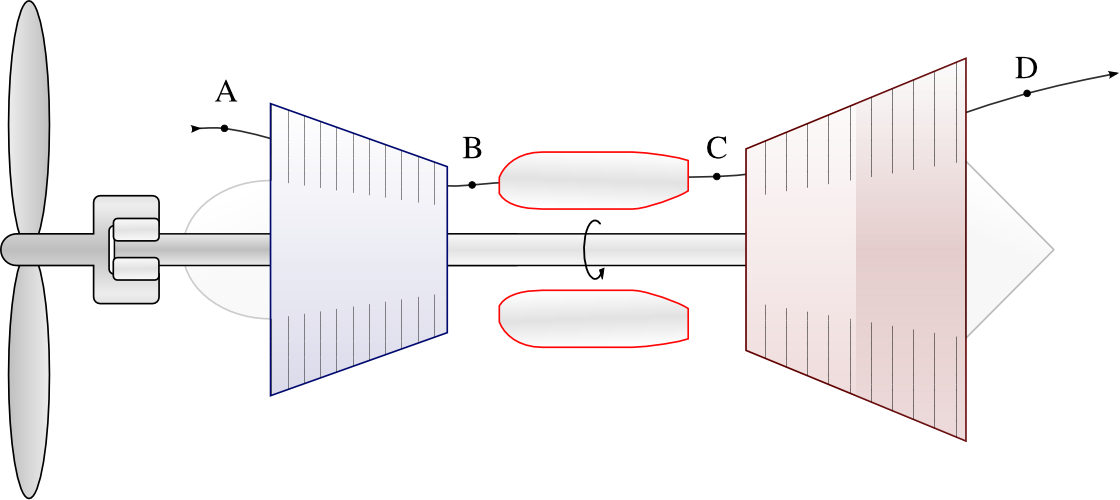
\includegraphics[width=12cm]{images/circuit_turboprop.png}
		\end{center}
		\supercaption{Schéma de principe d’un turbopropulseur. Ces moteurs sont étudiés plus en détail au \S\ref{ch_turboprop_turboshaft} p.\pageref{ch_turboprop_turboshaft}.}{schéma \ccbysa \olivier}
		\label{fig_turboprop}
	\end{figure}

	
	Au sein du compresseur, l’air se comporte de façon telle que ses propriétés suivent la relation $p \ v^{1,4} = k$, où $k$ est une constante.

	\begin{enumerate}
		\item Quelle est la puissance spécifique minimale à fournir au compresseur pour qu’il puisse fonctionner ?
		\item Représentez les propriétés du gaz lorsqu’il traverse le compresseur sur un diagramme pression-volume, de façon qualitative.
		\item Sur le schéma ci-dessus, représentez l’évolution que le gaz suivrait si le compresseur n’était pas réversible (compresseur réel, induisant un frottement interne au gaz) mais que l’on maintenait sa pression de sortie à~\SI{11}{\bar}.
	\end{enumerate}
	
	Au sein du même moteur, la turbine, qui est adiabatique, doit alimenter non seulement le compresseur mais aussi l’hélice à l’avant du moteur. Elle est munie de nombreuses sondes qui permettent de mesurer les propriétés de l’air.
	
	On mesure à l’entrée les propriétés suivantes :
		%\begin{tabularx}{10cm}{l S@{}s[table-unit-alignment = left]}
		%Pression 					& 11 	& \bar \\
		%Vitesse 						& 12 	& \metre\per\second \\
		%Volume spécifique 		& 0,36 	& \metre\cubed\per\kilogram \\
		%Énergie interne 			& 985,8 & \kilo\joule\per\kilogram \\
		%\end{tabularx}
	\begin{itemize}
		\item Pression 		\tab \SI{11}{\bar}
		\item Vitesse 		\tab \SI{12}{\metre\per\second}
		\item Volume spécifique 		\tab \SI{0,36}{\metre\cubed\per\kilogram}
		\item Énergie interne 		\tab \SI{985,8}{\kilo\joule\per\kilogram}
	\end{itemize}
	
	À la sortie les propriétés de l’air sont devenues :	
	\begin{itemize}
		\item Pression 		\tab \SI{0,8}{\bar}
		\item Vitesse 		\tab \SI{12}{\metre\per\second}
		\item Enthalpie spécifique 		\tab \SI{652,5}{\kilo\joule\per\kilogram}
	\end{itemize}

	\begin{enumerate}
		\shift{3}
		\item Quelle puissance spécifique la turbine développe-t-elle ?
		\item Quelle condition doit-on respecter au sein du moteur pour qu’il fournisse à l’hélice une puissance de~\SI{600}{\kilo\watt} ?
	\end{enumerate}

\exercisesolutionpage
\titreresultats

\begin{description}
	\item [\ref{exo_turbine_vapeur}]
					\tab 1) $w_\fromatob = \SI{-730,3}{\kilo\joule\per\kilogram}$
					\tab 2) $\dot m = \frac{\dot{W}_\fromatob}{w_\fromatob} = \SI{5,477}{\kilogram\per\second}$
	\item [\ref{exo_generatrice_electrique}]
					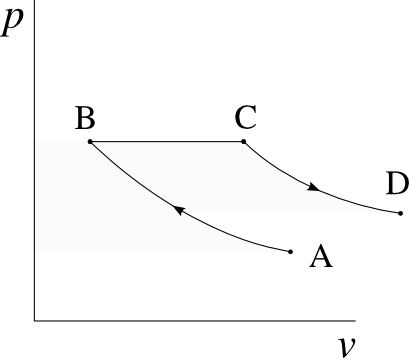
\includegraphics[width=\solutiondiagramwidth]{images/exo_sol_pv_1.png}
					\tab 1) $\dot{W}_\fromatob = \SI{+4,219}{\mega\watt}$
					\tab 2) $\dot{W}_\fromctod = \SI{-6,349}{\mega\watt}$
					\tab 3) $\dot{E}_\text{génératrice} = \eta_\text{génératrice} \eta_\text{transmission} \left(\dot{W}_\fromatob + \dot{W}_\fromctod\right) = \SI{-1,774}{\mega\watt}$
					\tab 5) $\dot{Q}_\text{refroidissement} = - \dot{W}_\fromatob - \dot{Q}_\text{combustion} - \dot{W}_\fromctod = \SI{-2,897}{\mega\watt}$ (soit plus de la moitié de la chaleur de combustion…)
	\item [\ref{exo_chaudiere_vapeur}]
					\tab 1) $\dot{m}_\text{déchets} \geq \SI{93,59}{\tonne\per\hour}$
	\item [\ref{exo_tuyere_turboreacteur}]
					\tab 1) $C_2 = \SI{624}{\metre\per\second}$ (environ \SI[per-mode=symbol]{2250}{\kilo\metre\per\hour}…)
					\tab 2) $\dot{V}_1 = \dot m \ v_1 = \SI{35,4}{\metre\cubed\per\second}$ \& $\dot{V}_2 = \SI{66,3}{\metre\cubed\per\second}$.
	\item [\ref{exo_turbine_eau}]
					\tab 1) $\dot{W}_\fromatob = \SI{-3,5}{\mega\watt}$
					\tab 2) $\dot{W}_{\fromatob2} = \SI{-6,45}{\mega\watt}$
	\item [\ref{exo_postcombustion}]
					\tab 1) \SI{+52}{\percent} par rapport à la poussée sèche ($C_{3\text{b}} = \SI{950,1}{\metre\per\second}$)
					\tab 2) $\dot{m}_\text{carburant} = \frac{\dot{m}_\text{air} \ q_{1\to 2\text{b}}}{q_\text{carburant}} = \SI[per-mode=symbol]{4157}{\kilogram\per\hour}$
					\tab 3) $\dot{V}_{3\text{b}} = \SI{145,9}{\metre\cubed\per\second} $
					\tab 4) $\eta_\text{postcombustion} = \frac{\frac{1}{2}\left(C_{3\text{b}}^2 - C_2^2\right)}{q_{1\to 2\text{b}}} =  \SI{19,3}{\percent}$ (raison pour laquelle elle n’est jamais utilisée sur les appareils civils)
	\item [\ref{exo_turbine_vapeur_2}]
					\tab 1) $\Delta e_c = \SI{+63}{\kilo\joule\per\kilogram}$, $\Delta e_p = \SI{+0,0294}{\kilo\joule\per\kilogram}$ (!), $\Delta h = \SI{-435,6}{\kilo\joule\per\kilogram}$.
					\tab 2) Dans l’équation~\ref{eq_petite_sfee_deltas_h}, imposer $q_{1 \to 2} = 0$ ne garantit pas que $w_{1 \to 2}$ augmentera. Il est probable que les conditions de sortie soient modifiées : les \SI{3}{\kilo\watt} seront au moins en partie retrouvés dans les $\Delta$ calculés ci-dessus.
	\item [\ref{exo_detente_turbine_turbomoteur}]
					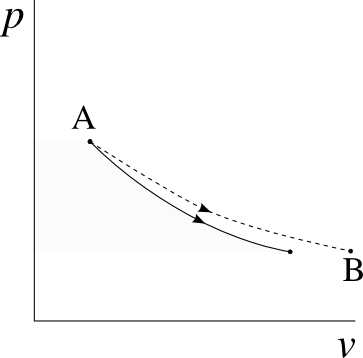
\includegraphics[width=\solutiondiagramwidth]{images/exo_sol_pv_2.png}
					\tab 1) cf. \S\ref{ch_reversibilite} p.\pageref{ch_reversibilite}
					\tab 2) $\dot{W}_\fromatob = \dot m k^{\frac{1}{\num{1,4}}} \left[\frac{1}{-\frac{1}{\num{1,4}} +1} p^{-\frac{1}{\num{1,4}} +1}\right]_{p_\A}^{p_\B} = \SI{-354,1}{\kilo\watt}$
					\tab 4) Sous forme de $\Delta h$ -- l’air de sortie aura un volume spécifique et une température (énergie interne) plus importants. Peut-être également sous forme d’énergie cinétique.
	\item [\ref{exo_compresseur_turbine_turbopropulseur}]
					\tab 1) $w_\fromatob \geq \int_\A^\B v \diff p = \SI{+312}{\kilo\joule\per\kilogram}$
					\tab 2) \& 3) cf. \cref{fig_pv_evolution_irr_so} p.\pageref{fig_pv_evolution_irr_so} ;
					\tab 4) $w_\fromctod = \SI{-729,3}{\kilo\joule\per\kilogram}$
					\tab 5) $\dot{m}_\text{air} = \frac{\dot{W}_\text{hélices}}{w_\text{hélices}} = \frac{\dot{W}_\text{hélices}}{w_\fromatob + w_\fromctod} = \SI{1,438}{\kilogram\per\second}$.
\end{description}
